\chapter{Policy Brief}

\begin{quote}
\textit{“Complex algorithms alone do not pass municipal ordinances. To transform predictive data into public action, computational science must speak the language of governance.”}
\end{quote}


This chapter presents the culminating artifact of this research: a comprehensive Policy Brief designed explicitly for the local executives, legislators, and environmental officers of the Municipality of Bacolod. 

While the preceding chapters of this thesis rigorously detail the mathematical validation, algorithmic training, and simulation outputs of the Deep Reinforcement Learning (DRL) models, academic research frequently suffers from an "implementation gap." Advanced computational models often remain confined to academic journals because their findings are not translated into accessible, actionable formats for non-technical decision-makers. 

The attached document outlines the proposed Data-Driven Solid Waste Management (DD-SWM) Framework. It summarizes the structural flaws of the status quo and delivers a clear, four-pillar roadmap to transition the Municipality of Bacolod from reactive enforcement to proactive, predictive smart-city governance.

% Include the first page of the PDF scaled to the full physical page
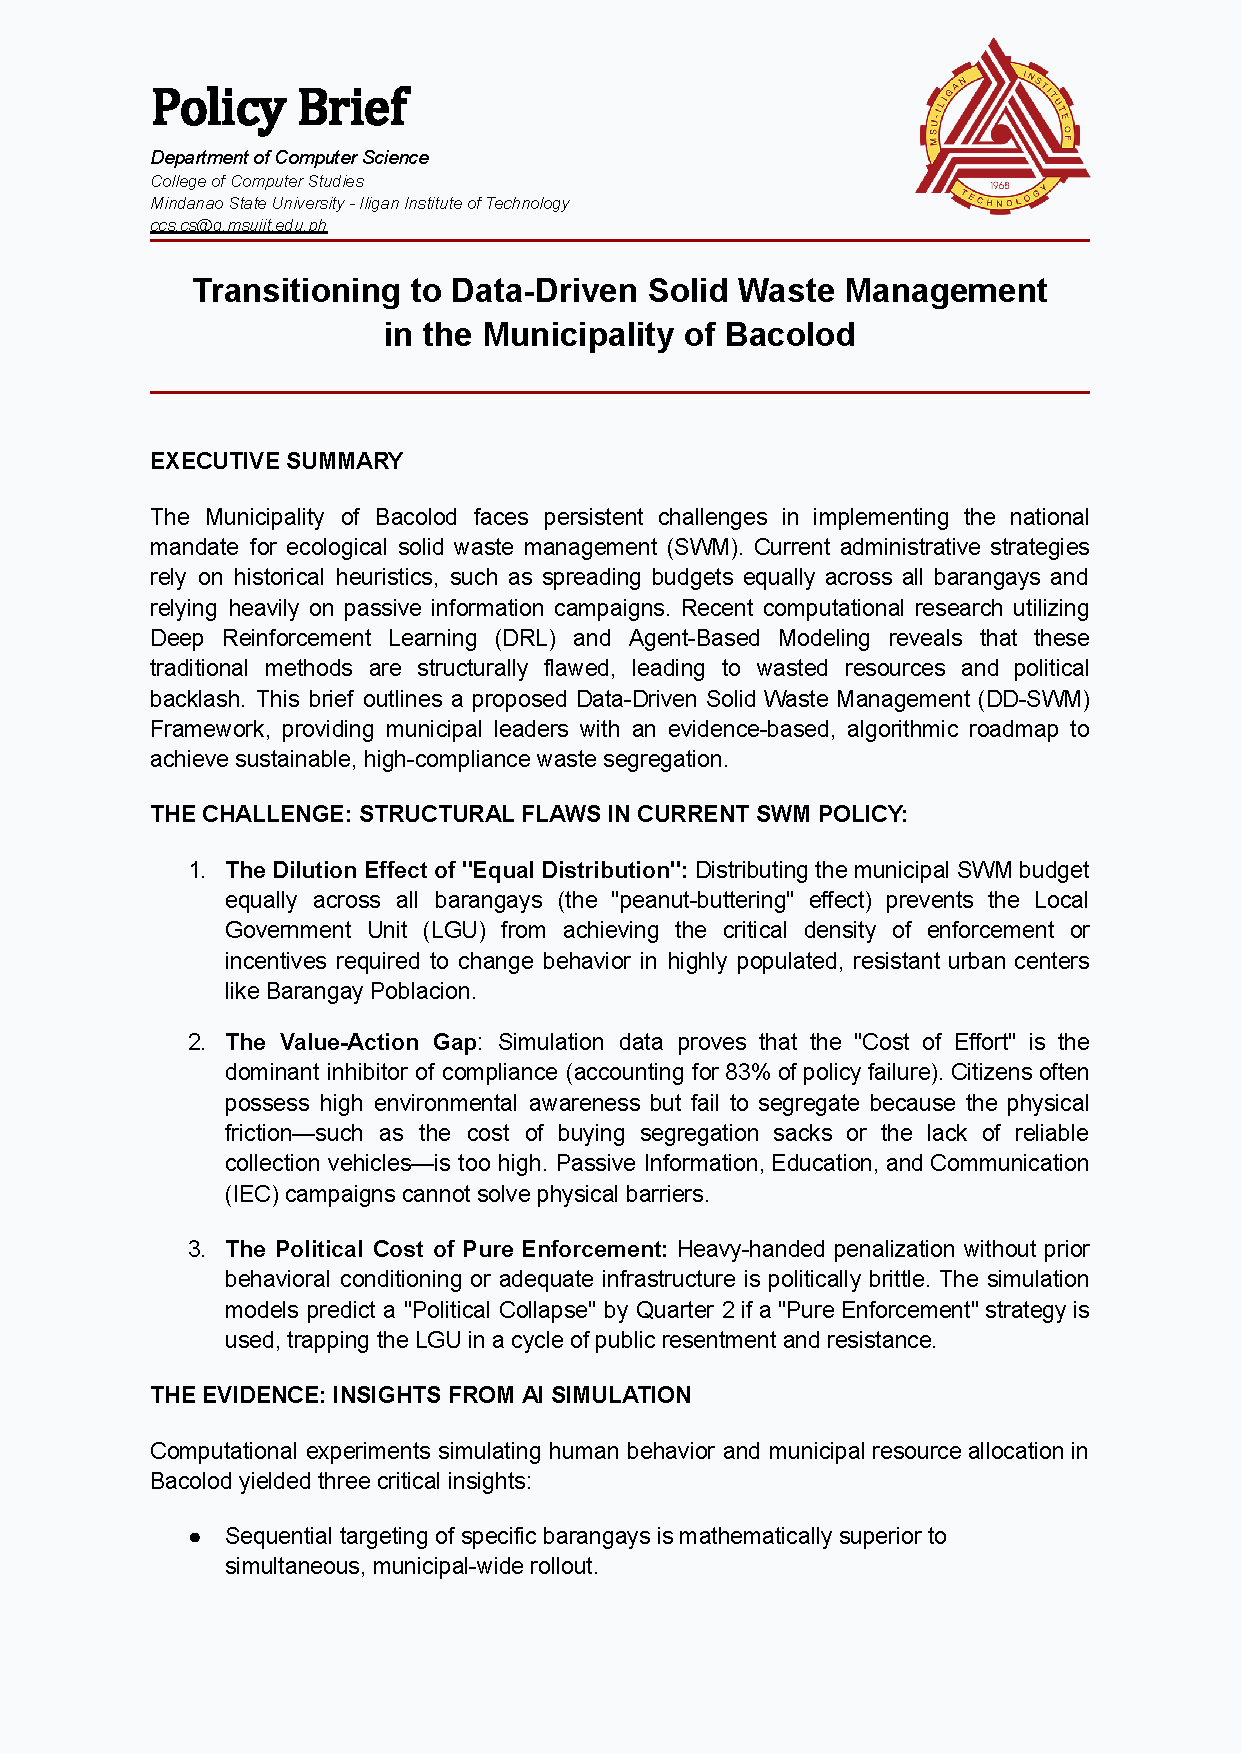
\includepdf[
    pages=1, 
    width=\paperwidth, 
    height=\paperheight, 
    keepaspectratio,
    pagecommand={
        \label{appendix:policy_brief}
        \thispagestyle{empty} 
    }
]{appD/policy_brief.pdf}

% Include the remaining pages scaled to the full physical page
\includepdf[
    pages=2-, 
    width=\paperwidth, 
    height=\paperheight, 
    keepaspectratio,
    pagecommand={\thispagestyle{empty}} 
]{appD/policy_brief.pdf}